\documentclass[11pt]{article}
\usepackage[margin=0.9in]{geometry}
\usepackage{amsmath,amssymb,amsthm,graphicx,microtype,enumitem}
\usepackage[hidelinks]{hyperref}

\newtheorem{theorem}{Theorem}
\newtheorem{lemma}[theorem]{Lemma}
\newtheorem{corollary}[theorem]{Corollary}
\theoremstyle{remark}
\newtheorem{remark}[theorem]{Remark}
\newcommand{\R}{\mathbb R}
\newcommand{\N}{\mathbb N}

\title{Gaussian kernels fail on every positive-dimensional\\closed Riemannian manifold}
\author{Candidate full result for arXiv:2303.06558}
\date{13 August 2026}

\begin{document}
\maketitle

\begin{center}
\fbox{\parbox{0.92\textwidth}{\textbf{Status.}
Candidate full result, likely valid.  We prove the qualitative extension
suggested in the source: for every positive-dimensional closed Riemannian
manifold, including every simply connected one, the intrinsic Gaussian kernel
is not positive definite at any positive bandwidth.}}
\end{center}

\section{Source question and result}

For a metric space $(X,d)$, write
\[
 \Lambda_+(X)=\{\lambda>0:e^{-\lambda d(\cdot,\cdot)^2}
 \text{ is positive definite}\}.
\]
Siran Li's source paper \cite{Li} proves that
$\Lambda_+(M,d_g)=\varnothing$ for every non-simply-connected closed
Riemannian manifold.  It records the suggestion that the same conclusion
should hold for \emph{every} closed Riemannian manifold, but says that it
cannot confirm the suggestion or provide a counterexample.  The exact passage
is reproduced in Figure~\ref{fig:source}.

\begin{figure}[ht]
\centering
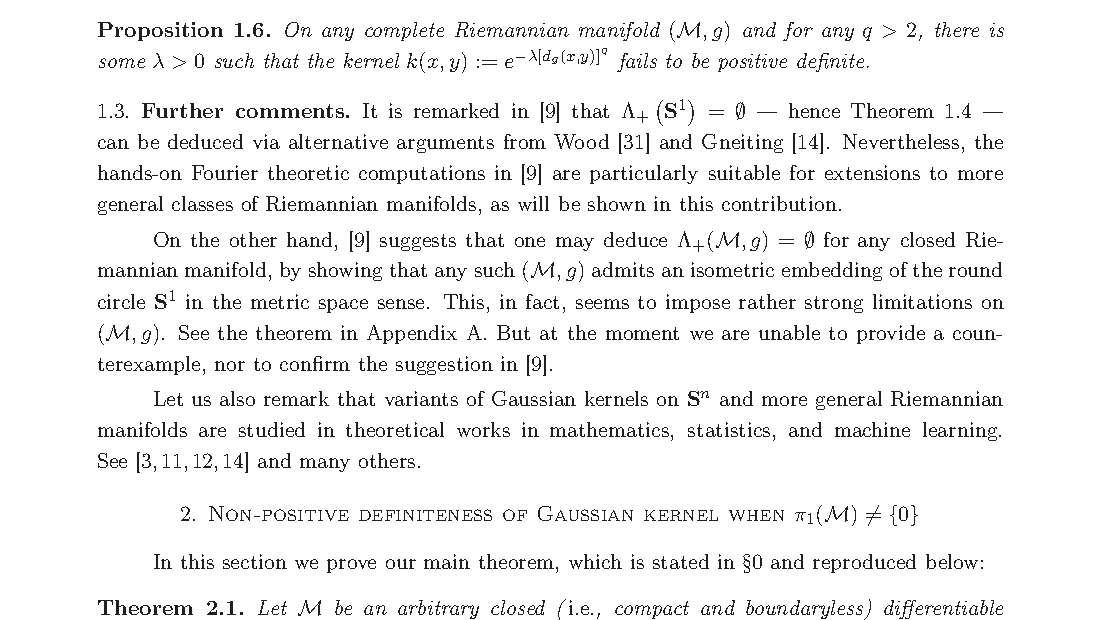
\includegraphics[width=0.94\textwidth]{figures/source_open_problem_crop.png}
\caption{The unresolved all-closed-manifolds suggestion on page 3 of the
official arXiv PDF.}
\label{fig:source}
\end{figure}

\noindent\textbf{Transcription of the source statement.}
``On the other hand, [9] suggests that one may deduce
$\Lambda_+(M,g)=\varnothing$ for any closed Riemannian manifold, by showing
that any such $(M,g)$ admits an isometric embedding of the round circle
$S^1$ in the metric space sense.  This, in fact, seems to impose rather
strong limitations on $(M,g)$.  See the theorem in Appendix A.  But at the
moment we are unable to provide a counterexample, nor to confirm the
suggestion in [9].''

\subsection*{Idea of the proof}
The source's obstruction uses a closed geodesic which is almost globally
distance minimizing.  Such control is unavailable in the simply connected
case.  The proof below instead uses only local minimality and the rigidity of
analytic positive-definite feature maps.  Along a short geodesic segment the
feature curve has exactly the line-Gaussian Gram matrix, which forces it to be
real analytic.  On a closed geodesic, analytic continuation is incompatible
with periodicity.

\begin{theorem}[full qualitative resolution]\label{thm:main}
Let $(M,g)$ be a positive-dimensional closed Riemannian manifold.  For every
$\lambda>0$, the kernel
\[
 k_\lambda(x,y)=\exp\!\bigl(-\lambda d_g(x,y)^2\bigr)
\]
is not positive definite.  Equivalently,
\[
 \boxed{\Lambda_+(M,d_g)=\varnothing.}
\]
\end{theorem}

We prove a metric obstruction which makes the mechanism transparent.

\section{The line-Gaussian feature curve}

Fix $\lambda>0$.  Define $\psi_\lambda:\R\to\ell^2(\N_0;\R)$ by
\begin{equation}\label{eq:psi}
 \bigl(\psi_\lambda(t)\bigr)_n
 =e^{-\lambda t^2}\frac{(2\lambda)^{n/2}t^n}{\sqrt{n!}},
 \qquad n\geq0.
\end{equation}
The exponential series gives
\begin{equation}\label{eq:gram}
 \langle\psi_\lambda(s),\psi_\lambda(t)\rangle
 =e^{-\lambda(s^2+t^2)}e^{2\lambda st}
 =e^{-\lambda(s-t)^2}.
\end{equation}

This curve is real analytic in Hilbert norm.  More explicitly, for $z\in
\mathbb C$ the same formula defines a vector in $\ell^2(\N_0;\mathbb C)$ and
\begin{equation}\label{eq:complexnorm}
 \sum_{n\geq0}\left|e^{-\lambda z^2}
 \frac{(2\lambda)^{n/2}z^n}{\sqrt{n!}}\right|^2
 =e^{-2\lambda\operatorname{Re}(z^2)+2\lambda|z|^2}
 =e^{4\lambda(\operatorname{Im}z)^2}.
\end{equation}
Thus the series converges locally uniformly in Hilbert norm and is an entire
$\ell^2(\mathbb C)$-valued map.

\begin{lemma}[local Gram rigidity]\label{lem:analytic}
Let $I\subset\R$ be an open interval and $F:I\to H$ a map into a real Hilbert
space such that
\[
 \langle F(s),F(t)\rangle_H=e^{-\lambda(s-t)^2}
 \qquad(s,t\in I).
\]
Then $F$ is real analytic in Hilbert norm.
\end{lemma}

\begin{proof}
On the algebraic span of $\{\psi_\lambda(t):t\in I\}$ define
\[
 U\!\left(\sum_j a_j\psi_\lambda(t_j)\right)=\sum_j a_jF(t_j).
\]
The asserted equality of Gram matrices shows that the two sides always have
the same squared norm.  Hence $U$ is well defined and isometric, and it
extends to the closed span.  In particular,
$F(t)=U\psi_\lambda(t)$ on $I$.  Equations \eqref{eq:psi}--\eqref{eq:complexnorm}
now prove Hilbert-norm real analyticity.
\end{proof}

\section{Periodic local geodesics are impossible}

Call a map $\gamma:\R\to(X,d)$ a \emph{periodic local unit geodesic} if it
has a period $L>0$ and, for every $a\in\R$, there is an open interval $I_a$
containing $a$ such that
\begin{equation}\label{eq:localisometry}
 d(\gamma(s),\gamma(t))=|s-t|\qquad(s,t\in I_a).
\end{equation}

\begin{lemma}[periodic-geodesic obstruction]\label{lem:periodic}
If a metric space contains a periodic local unit geodesic, then
$e^{-\lambda d^2}$ is not positive definite for any $\lambda>0$.
\end{lemma}

\begin{proof}
Suppose the kernel is positive definite.  By the standard feature-map
construction there are a real Hilbert space $H$ and a map $\Phi:X\to H$ with
\begin{equation}\label{eq:feature}
 \langle\Phi(x),\Phi(y)\rangle_H=e^{-\lambda d(x,y)^2}.
\end{equation}
Set $F=\Phi\circ\gamma$.  On every interval $I_a$, equations
\eqref{eq:localisometry} and \eqref{eq:feature} give the hypothesis of
Lemma~\ref{lem:analytic}.  Therefore $F:\R\to H$ is locally, hence globally,
real analytic.

Fix $a\in\R$.  The scalar function
\[
 h_a(t)=\langle F(a),F(t)\rangle_H
\]
is real analytic on the connected line.  On a neighborhood of $a$, local
minimality gives
\[
 h_a(t)=e^{-\lambda(t-a)^2}.
\]
The identity theorem for real-analytic functions forces this equality for
every $t\in\R$.  But $\gamma(a+L)=\gamma(a)$, so \eqref{eq:feature} yields
\[
 1=\|F(a)\|^2=h_a(a+L)=e^{-\lambda L^2}<1,
\]
a contradiction.
\end{proof}

\section{Application to closed manifolds}

\begin{proof}[Proof of Theorem~\ref{thm:main}]
The Lyusternik--Fet theorem \cite{LF} states that every
positive-dimensional closed Riemannian manifold has a nonconstant closed
geodesic.  Parametrize one by unit speed and lift its periodic parameter to
$\gamma:\R\to M$, with period equal to its positive length.  Every
Riemannian geodesic is distance minimizing on sufficiently short parameter
intervals.  Thus $\gamma$ satisfies \eqref{eq:localisometry}, and
Lemma~\ref{lem:periodic} excludes positive definiteness for the arbitrary
parameter $\lambda>0$.
\end{proof}

The same proof applies to any metric space with a periodic local unit
geodesic; neither a globally isometrically embedded round circle nor a
globally shortest closed geodesic is needed.  This is exactly why the
argument crosses the simple-connectivity barrier identified in the source.

\section{Verification, novelty, and boundary}

The included verifier checks finite truncations of \eqref{eq:psi} against the
exact Gram identity \eqref{eq:gram} and evaluates the strictly positive
separation
\[
 \|\psi_\lambda(0)-\psi_\lambda(L)\|^2
 =2\bigl(1-e^{-\lambda L^2}\bigr)>0,
\]
which periodicity would force to vanish.  The mathematical audit in
\texttt{VERIFIER\_REPORT.md} separately checks feature-map existence, the
local Gram isometry, Hilbert-valued analyticity, scalar continuation, and the
Lyusternik--Fet reduction.

Bounded searches of the run indexes, the exact source suggestion, later
citations, and combinations of ``Gaussian kernel'', ``closed geodesic'', and
``analytic continuation'' through 13 August 2026 found no later proof.  A
2025 experimental study still presents the geometry-versus-bandwidth problem
as open.  Novelty confidence is high enough for promotion but remains subject
to expert literature review, especially for prior general theorems propagating
near-diagonal analyticity of positive-definite kernels.

Dimension zero is essential: as the source notes, finite metric spaces can
have a nonempty proper positivity range.  The result settles the qualitative
closed-manifold conclusion.  It does not quantify how many sample points, or
what spacing, is needed to exhibit a negative Gram eigenvalue at a fixed
$\lambda$; that finite-scale problem remains open.

\noindent\textbf{Human-review recommendation.}
Audit Lemma~\ref{lem:analytic}'s Gram-isometry construction and the use of the
real-analytic identity theorem in Lemma~\ref{lem:periodic}.  Then perform a
specialist search in the regularity theory of positive-definite kernels before
asserting priority.

\begin{thebibliography}{9}
\bibitem{Li}
S. Li,
\emph{Gaussian kernels on non-simply-connected closed Riemannian manifolds
are never positive definite}, Bull. Lond. Math. Soc. \textbf{56} (2024),
263--273; arXiv:2303.06558.

\bibitem{LF}
L. A. Lyusternik and A. I. Fet,
\emph{Variational problems on closed manifolds}, Dokl. Akad. Nauk SSSR
(N.S.) \textbf{81} (1951), 17--18 (in Russian).
\end{thebibliography}

\end{document}
